%% =====================================================================
%% Slide báo cáo BTL Hệ thống và mạng máy tính (MI4060)
%% Theme: HUST Beamer (bản fork vanetta), biên dịch bằng LuaLaTeX + Biber
%%   lualatex -shell-escape slide_baocao  ->  biber slide_baocao  ->  lualatex x2
%% Số liệu lấy từ báo cáo LaTeX (GraduationThesisTemplate-main) và data/*.csv
%% =====================================================================
\documentclass[aspectratio=169,10pt]{beamer}

\usetheme[
  color=blue,
  font=lato,
  titlefont=avantgarde,
  footerlogo=mark,
  bar=thin,
  titlepage=cover,
  sectionpage=panel,
  numbering=fraction,
  progressbar=on,
  dateaddress=on,
  address={Hà Nội},
  logolayout=2,
  framebg=on,
  footermeta=on,
  footertitle={Federated Learning trên nền tảng Mininet},
  toctitle={Nội dung trình bày}
]{HUST}

%% ==============================================================================
%% HUST Beamer Theme - Setup & Academic Extension Package (hust-setup.tex)
%% Modular setup file containing academic packages, UX/UI extensions,
%% math operators, list customizations, and cross-references.
%% ==============================================================================

%% ------------------------------------------------------------- 1. Layout & Tables
\RequirePackage{wrapfig}
\RequirePackage{booktabs}
\RequirePackage{tabularx}
\RequirePackage{multirow, multicol}
\RequirePackage{array}
\renewcommand{\tabularxcolumn}[1]{m{#1}}
\RequirePackage{caption}
\captionsetup{font=scriptsize, labelfont={bf, color=hustmain}, labelsep=colon}

%% TikZ libraries for graphics & markers:
\usetikzlibrary{calc, decorations.markings, arrows.meta}

%% ------------------------------------------------------------- 2. List Customization (enumitem & tasks)
\RequirePackage{enumitem}
%% Safe reconfiguration to avoid Beamer labelenumi recursion:
\setlist[enumerate,1]{label=\arabic*.}
\setlist[enumerate,2]{label=\alph*.}
\setlist[enumerate,3]{label=\roman*)}
\setlist[itemize,1]{label=\usebeamerfont*{itemize item}\usebeamercolor[fg]{itemize item}\raise0.2ex\hbox{\vrule height 0.8ex width 0.8ex}}
\setlist[itemize,2]{label=\usebeamerfont*{itemize subitem}\usebeamercolor[fg]{itemize subitem}\raise0.2ex\hbox{\vrule height 0.6ex width 0.6ex}}
\setlist[itemize,3]{label=\raisebox{0.2ex}{\tiny\textcolor{hustaccent}{$\bullet$}}}
\setlist[itemize,4]{label=\raisebox{0.2ex}{\tiny\textcolor{hustmain}{$-$}}}

%% Square number box badge matching HUST Brand identity:
\DeclareRobustCommand{\hustitemsq}[1]{%
  \raisebox{0.05ex}{\colorbox{hustmain}{\makebox[1.05em]{\textcolor{white}{\bfseries\scriptsize#1}}}}%
}

%% Dedicated square-numbered list environment:
\newlist{hustsqlist}{enumerate}{2}
\setlist[hustsqlist,1]{label=\hustitemsq{\arabic*}, ref=\arabic*, leftmargin=2.2em, labelsep=0.6em, itemsep=4pt, topsep=2pt}
\setlist[hustsqlist,2]{label=\hustitemsq{\alph*}, ref=\alph*, leftmargin=2.2em, labelsep=0.6em, itemsep=3pt, topsep=2pt}

%% Tasks package for multi-column horizontal listings:
%% Default task behavior uses the standard Beamer itemize square bullet.
%% To use square letter badges, pass [label=\hustitemsq{\alph*}, label-width=1.5em, item-indent=1.9em].
\RequirePackage{tasks}
\settasks{
  before-skip = 2pt,
  after-skip = 2pt,
  after-item-skip = 3pt,
  label-width = 5pt,
  item-indent = 9pt,
  label-offset = 2pt,
  column-sep = 1em,
  ref = \arabic*,
  label = \raisebox{0.15ex}{\textcolor{hustmain}{\rule{0.75ex}{0.75ex}}}
}

%% ------------------------------------------------------------- 3. Mathematics & Operators
\RequirePackage{amsmath, mathtools}
\RequirePackage{derivative}
\RequirePackage{nicematrix, nicefrac}
\RequirePackage{siunitx}

%% Bold math compatibility:
\ifdefined\symbfit
  \providecommand{\bm}[1]{\symbfit{#1}}
\else
  \providecommand{\bm}[1]{\boldsymbol{#1}}
\fi

%% Contour integrals & symbols:
\providecommand{\oiint}{\oint\mkern-13mu\oint}
\providecommand{\ointctrclockwise}{\oint}

%% Pre-defined paired delimiters:
\DeclarePairedDelimiter{\abs}{\lvert}{\rvert}
\DeclarePairedDelimiter{\norm}{\lVert}{\rVert}
\DeclarePairedDelimiter{\innerp}{\langle}{\rangle}
\DeclarePairedDelimiter{\ceil}{\lceil}{\rceil}
\DeclarePairedDelimiter{\floor}{\lfloor}{\rfloor}

%% Math operators:
\DeclareMathOperator*{\argmin}{arg\,min}
\DeclareMathOperator*{\argmax}{arg\,max}
\DeclareMathOperator*{\Arg}{Arg}
\DeclareMathOperator*{\Real}{Re}
\DeclareMathOperator*{\Image}{Img}

%% Stretchy arrows:
\newcommand{\vv}[1]{\overrightarrow{#1}}
\newcommand{\vs}[1]{\vec{#1}}

%% ------------------------------------------------------------- 4. Cleveref & Cross-referencing
\makeatletter
%% Trick cleveref into enabling full hyperref link support in Beamer:
\expandafter\let\csname opt@hyperref.sty\endcsname\@empty
\makeatother
\RequirePackage{cleveref}

\makeatletter
%% Synchronize external links to hustmain color:
\let\hust@orig@href\href
\renewcommand{\href}[2]{\hust@orig@href{#1}{\textcolor{hustmain}{#2}}}

%% Ensure \eqref creates a clickable link in Beamer:
\renewcommand{\eqref}[1]{\hyperref[#1]{\textcolor{hustmain}{\textup{(\ref*{#1})}}}}

%% Cleveref name definitions & clickable format:
\crefname{equation}{phương trình}{phương trình}
\Crefname{equation}{Phương trình}{Phương trình}
\crefformat{equation}{#2\textcolor{hustmain}{phương trình~#1}#3}
\Crefformat{equation}{#2\textcolor{hustmain}{Phương trình~#1}#3}

\crefname{figure}{hình}{hình}
\Crefname{figure}{Hình}{Hình}
\crefformat{figure}{#2\textcolor{hustmain}{hình~#1}#3}
\Crefformat{figure}{#2\textcolor{hustmain}{Hình~#1}#3}

\crefname{table}{bảng}{bảng}
\Crefname{table}{Bảng}{Bảng}
\crefformat{table}{#2\textcolor{hustmain}{bảng~#1}#3}
\Crefformat{table}{#2\textcolor{hustmain}{Bảng~#1}#3}

\crefname{section}{mục}{mục}
\Crefname{section}{Mục}{Mục}
\crefformat{section}{#2\textcolor{hustmain}{mục~#1}#3}
\Crefformat{section}{#2\textcolor{hustmain}{Mục~#1}#3}

\crefname{subsection}{mục}{mục}
\Crefname{subsection}{Mục}{Mục}
\crefformat{subsection}{#2\textcolor{hustmain}{mục~#1}#3}
\Crefformat{subsection}{#2\textcolor{hustmain}{Mục~#1}#3}

\crefname{hustsqlisti}{mục}{mục}
\Crefname{hustsqlisti}{Mục}{Mục}
\crefformat{hustsqlisti}{#2\textcolor{hustmain}{mục~#1}#3}
\Crefformat{hustsqlisti}{#2\textcolor{hustmain}{Mục~#1}#3}

\crefname{algocf}{thuật toán}{thuật toán}
\Crefname{algocf}{Thuật toán}{Thuật toán}
\crefformat{algocf}{#2\textcolor{hustmain}{thuật toán~#1}#3}
\Crefformat{algocf}{#2\textcolor{hustmain}{Thuật toán~#1}#3}

\crefname{lstlisting}{đoạn mã}{đoạn mã}
\Crefname{lstlisting}{Đoạn mã}{Đoạn mã}
\crefformat{lstlisting}{#2\textcolor{hustmain}{đoạn mã~#1}#3}
\Crefformat{lstlisting}{#2\textcolor{hustmain}{Đoạn mã~#1}#3}

\crefname{listing}{đoạn mã}{đoạn mã}
\Crefname{listing}{Đoạn mã}{Đoạn mã}
\crefformat{listing}{#2\textcolor{hustmain}{đoạn mã~#1}#3}
\Crefformat{listing}{#2\textcolor{hustmain}{Đoạn mã~#1}#3}

\crefname{theorem}{định lý}{định lý}
\Crefname{theorem}{Định lý}{Định lý}
\crefformat{theorem}{#2\textcolor{hustmain}{định lý~#1}#3}
\Crefformat{theorem}{#2\textcolor{hustmain}{Định lý~#1}#3}

\crefname{definition}{định nghĩa}{định nghĩa}
\Crefname{definition}{Định nghĩa}{Định nghĩa}
\crefformat{definition}{#2\textcolor{hustmain}{định nghĩa~#1}#3}
\Crefformat{definition}{#2\textcolor{hustmain}{Định nghĩa~#1}#3}

\crefname{lemma}{bổ đề}{bổ đề}
\Crefname{lemma}{Bổ đề}{Bổ đề}
\crefformat{lemma}{#2\textcolor{hustmain}{bổ đề~#1}#3}
\Crefformat{lemma}{#2\textcolor{hustmain}{Bổ đề~#1}#3}

\crefname{corollary}{hệ quả}{hệ quả}
\Crefname{corollary}{Hệ quả}{Hệ quả}
\crefformat{corollary}{#2\textcolor{hustmain}{hệ quả~#1}#3}
\Crefformat{corollary}{#2\textcolor{hustmain}{Hệ quả~#1}#3}

\crefname{example}{ví dụ}{ví dụ}
\Crefname{example}{Ví dụ}{Ví dụ}
\crefformat{example}{#2\textcolor{hustmain}{ví dụ~#1}#3}
\Crefformat{example}{#2\textcolor{hustmain}{Ví dụ~#1}#3}

%% 4.1. Universal Figure / Table Custom Caption & Cross-Reference Engine
%% Supports:
%%   - Custom prefix name (e.g. Hình, Bảng, Figure, Table, Image, ...)
%%   - Auto-incrementing numbering per prefix or manual numbering (e.g. Hình 6, Bảng 2.5)
%%   - Clickable \cref / \Cref synchronization in hustmain color
\newcommand{\hustfigurename}{Hình}
\newcommand{\husttablename}{Bảng}
\newcommand{\hustsetfigurename}[1]{\renewcommand{\hustfigurename}{#1}}
\newcommand{\hustsettablename}[1]{\renewcommand{\husttablename}{#1}}

\newcounter{hustref}
\crefname{hustref}{}{}
\Crefname{hustref}{}{}
\crefformat{hustref}{#2\textcolor{hustmain}{#1}#3}
\Crefformat{hustref}{#2\textcolor{hustmain}{#1}#3}

\NewDocumentCommand{\hustcaption}{ O{\hustfigurename} o m }{%
  \par\vspace{3pt}\noindent
  \phantomsection
  \edef\hust@cap@name{#1}%
  \IfValueTF{#2}{%
    %% Manual numbering passed (e.g. [6], [2.5])
    \edef\hust@cap@num{#2}%
  }{%
    %% Auto-incremental numbering per custom name
    \@ifundefined{c@hust@cnt@\hust@cap@name}{%
      \newcounter{hust@cnt@\hust@cap@name}%
    }{}%
    \stepcounter{hust@cnt@\hust@cap@name}%
    \edef\hust@cap@num{\arabic{hust@cnt@\hust@cap@name}}%
  }%
  %% Setup labels for standard \ref and \cref / \Cref:
  \def\thehustref{\hust@cap@name~\hust@cap@num}%
  \refstepcounter{hustref}%
  %% Render caption centered matching HUST typography:
  \begin{center}
    {\scriptsize\bfseries\color{hustmain}\hust@cap@name~\hust@cap@num:}\ %
    {\normalfont\scriptsize #3}%
  \end{center}%
  \par\vspace{2pt}%
}
\makeatother

%% ------------------------------------------------------------- 5. Code & Pseudocode
\RequirePackage{listings}
\RequirePackage[linesnumbered,ruled,vlined]{algorithm2e}
\RequirePackage[highlightmode=immediate]{minted}

%% Keep algorithm2e line numbers and Input/Output strictly aligned inside the ruled block:
\SetNlSkip{0.5em}
\AtBeginEnvironment{algorithm}{%
  \IncMargin{1.2em}%
  \SetKwInput{KwIn}{\kern-1.2em Input}%
  \SetKwInput{KwOut}{\kern-1.2em Output}%
}

\makeatletter
\AtBeginDocument{%
  \renewcommand{\fnum@lstlisting}{Listing~\thelstlisting}%
}
\makeatother

\colorlet{hustcodebg}{hustmain!5!white}
\lstdefinestyle{hustcode}{
  backgroundcolor=\color{hustcodebg},
  basicstyle=\ttfamily\scriptsize,
  keywordstyle=\bfseries\color{hustmain},
  stringstyle=\color{HUSTOrange},
  commentstyle=\itshape\color{HUSTGray},
  numberstyle=\tiny\color{HUSTGray},
  numbers=left,
  numbersep=5pt,
  framesep=3pt,
  xleftmargin=1.5em,
  framexleftmargin=\dimexpr 1.5em - 3.5pt\relax,
  xrightmargin=3.5pt,
  framexrightmargin=0pt,
  frame=single,
  framerule=0.5pt,
  rulecolor=\color{hustmain!30},
  breaklines=true,
  tabsize=2,
  showstringspaces=false
}

%% Configure minted to match theme colors and keep line numbers inside the frame box:
\setminted{
  fontsize=\scriptsize,
  linenos=true,
  numbersep=5pt,
  xleftmargin=1.2em,
  breaklines=true,
  tabsize=2,
  frame=lines,
  framerule=0.5pt,
  rulecolor=\color{hustmain!40}
}
\renewcommand{\theFancyVerbLine}{\textcolor{HUSTGray}{\tiny\arabic{FancyVerbLine}}}

%% ------------------------------------------------------------- 5. Beamer Theorems & Academic Blocks
%% Enable numbering for Beamer theorem and definition environments:
\setbeamertemplate{theorems}[numbered]

%% Vietnamese localization for standard Beamer theorem environments:
\deftranslation{Definition}{Định nghĩa}
\deftranslation{Theorem}{Định lý}
\deftranslation{Lemma}{Bổ đề}
\deftranslation{Corollary}{Hệ quả}
\deftranslation{Example}{Ví dụ}
\deftranslation{Examples}{Ví dụ}
\deftranslation{Proof}{Chứng minh}
\deftranslation[to=English]{Definition}{Định nghĩa}
\deftranslation[to=English]{Theorem}{Định lý}
\deftranslation[to=English]{Lemma}{Bổ đề}
\deftranslation[to=English]{Corollary}{Hệ quả}
\deftranslation[to=English]{Example}{Ví dụ}
\deftranslation[to=English]{Examples}{Ví dụ}
\deftranslation[to=English]{Proof}{Chứng minh}
\providecommand{\proofname}{Chứng minh}
\renewcommand{\proofname}{Chứng minh}

%% Vector warning icon:
\DeclareRobustCommand{\warning}{%
  \tikz[baseline=0pt]{%
    \draw[line width=0.6pt, line join=round, draw=HUSTRed, fill=HUSTYellow!70, inner sep=0pt]
      (0,0) -- (1.1em,0) -- (0.55em,0.95em) -- cycle;
    \node[font=\tiny\bfseries, text=HUSTRed] at (0.55em,0.3em) {!};
  }\xspace}



%% End of hust-setup.tex


\usepackage{pgfplots}
\pgfplotsset{compat=1.17}
\usetikzlibrary{positioning, shapes.geometric, fit, backgrounds, decorations.pathreplacing}

\usepackage[backend=biber,style=numeric,sorting=none,maxcitenames=2,mincitenames=1]{biblatex}
\addbibresource{refs.bib}

%% Ô số liệu nổi bật
\newcommand{\kpi}[2]{%
  \begin{minipage}[t]{\linewidth}\centering
    {\LARGE\bfseries\color{hustmain}#1}\par\vspace{2pt}
    {\scriptsize #2}
  \end{minipage}}

\title[Federated Learning trên nền tảng Mininet]{%
  {\normalsize BÁO CÁO BÀI TẬP LỚN MI4060}\\[5pt]
  {\bfseries Federated Learning\\trên nền tảng Mininet}}
\subtitle{Tự động hóa đo lường \& Đánh giá hiệu năng mạng}
\author[Nhóm 1]{Nhóm 1: Hứa Ngọc Khánh -- Nguyễn Đức Chung\\ Nguyễn Hữu Kiến -- Phí Việt Hiếu\\ Đoàn Hữu Việt -- Nguyễn Việt Hùng\\ GVHD: Ngô Thị Hiền}
\institute{Hướng 2: Networking for AI\\Đại học Bách khoa Hà Nội}
\date{\today}

\begin{document}

%% ---------------------------------------------------------------------
\hustsetup{slogantext={}}
\begin{frame}[plain,noframenumbering]
  \titlepage
\end{frame}

\begin{frame}[noprogressbar]{\husttoctitle}{\husttocsubtitle}
  \tableofcontents[split=4,hideallsubsections]
\end{frame}

%% =====================================================================
\section{Đặt vấn đề}
%% =====================================================================

\begin{frame}{Federated Learning nhìn từ phía mạng}{Dữ liệu không rời thiết bị, nhưng trọng số mô hình phải đi qua mạng mỗi vòng}
  \begin{columns}[T]
    \begin{column}{0.52\textwidth}
      \textbf{Một vòng FedAvg}~\cite{mcmahan2017fedavg} gồm 4 bước:
      \begin{enumerate}
        \item Aggregator phát mô hình $w_t$ xuống $N$ Edge Node
        \item Mỗi node huấn luyện cục bộ
        \item Node gửi trọng số mới về Aggregator
        \item Tổng hợp: $w_{t+1} = \sum_k \frac{n_k}{n}\, w^{k}_{t+1}$
      \end{enumerate}
      \vspace{4pt}
      \begin{alertblock}{Vấn đề}
        Mỗi vòng có $2N \cdot S$ byte đi qua \textbf{giao diện mạng của Aggregator}; vòng chỉ kết thúc khi bản cập nhật \emph{cuối cùng} tới nơi.
      \end{alertblock}
    \end{column}
    \begin{column}{0.44\textwidth}
      \centering
      \begin{tikzpicture}[
          n/.style={draw, rounded corners, fill=hustmain!10, minimum width=1.0cm, minimum height=0.6cm, font=\scriptsize},
          a/.style={draw, rounded corners, fill=HUSTOrange!20, minimum width=2.4cm, minimum height=0.8cm, font=\scriptsize, align=center},
          dn/.style={-{Stealth[length=2mm]}, thick, hustmain},
          up/.style={-{Stealth[length=2mm]}, thick, HUSTOrange}]
        \node[a] (agg) at (0,2.6) {Aggregator\\(FedAvg)};
        \foreach \i/\x in {1/-2.1,2/-0.7,3/0.7,4/2.1} {
          \node[n] (h\i) at (\x,0) {Node \i};
          \draw[dn] ([xshift=-3pt]agg.south) to[bend right=8] ([xshift=-3pt]h\i.north);
          \draw[up] ([xshift=3pt]h\i.north) to[bend right=8] ([xshift=3pt]agg.south);
        }
        \node[font=\scriptsize, hustmain] at (-2.3,1.6) {$w_t$ ($S$ byte)};
        \node[font=\scriptsize, HUSTOrange] at (2.3,1.6) {$w^{k}_{t+1}$};
        \node[font=\scriptsize, align=center] at (0,-0.9) {Điểm nghẽn tự nhiên: link vào Aggregator};
      \end{tikzpicture}
      \vspace{6pt}

      \scriptsize Mô hình nặng vài MB tới hàng trăm MB: thời gian truyền thường lớn hơn thời gian tính toán~\cite{konecny2016communication}.
    \end{column}
  \end{columns}
\end{frame}

\begin{frame}{Mục tiêu và ba câu hỏi nghiên cứu}{Định lượng chi phí truyền thông của một vòng đồng bộ FL trên mạng Edge--Cloud}
  \small
  \begin{tabularx}{\textwidth}{>{\raggedright\arraybackslash\hsize=1.1\hsize}X >{\raggedright\arraybackslash\hsize=0.9\hsize}X}
    \toprule
    \textbf{Câu hỏi} & \textbf{Chỉ số đo} \\
    \midrule
    \textbf{Q1.} Băng thông biên 1--100~Mbps tác động thế nào đến thời gian một vòng FL? & $T_{round}$, $T_{down}$, $T_{up}$; thông lượng gộp; RTT khi có tải; số nút $N$ \\
    \midrule
    \textbf{Q2.} Mất gói 0--5\% và độ trễ WAN ảnh hưởng thế nào đến sự hội tụ? & Độ chính xác theo vòng; số vòng và thời gian tới 90\% (TTA) \\
    \midrule
    \textbf{Q3.} FLSync/TCP tốn bao nhiêu overhead; nén 1/10 và tổng hợp tại biên hiệu quả đến đâu? & Hiệu suất byte; ACK, header, truyền lại; $T_{round}$ Edge vs Cloud \\
    \bottomrule
  \end{tabularx}
  \vspace{8pt}

  \begin{block}{Phương pháp}
    \textbf{(1)} Giả lập mạng Edge--Cloud trên Mininet và đo tự động \quad
    \textbf{(2)} Bắt gói tcpdump/Wireshark để giải thích số đo
  \end{block}
\end{frame}

%% =====================================================================
\section{Cơ sở lý thuyết mạng}
%% =====================================================================

\begin{frame}{Kiến trúc Edge--Cloud: đặt nút tổng hợp ở đâu?}{Hai vị trí được dựng trên cùng một topo để so sánh trực tiếp}
  \begin{columns}[T]
    \begin{column}{0.50\textwidth}
      \small
      \begin{tabular}{l l l}
        \toprule
        \textbf{Tiêu chí} & \textbf{Tại biên} & \textbf{Trên cloud} \\
        \midrule
        Vị trí & cùng LAN & sau chặng WAN \\
        RTT & vài ms & hàng chục ms+ \\
        Băng thông & bằng LAN & giới hạn bởi WAN \\
        Tài nguyên & hạn chế & lớn \\
        Phạm vi & một vùng & mọi vùng \\
        \bottomrule
      \end{tabular}
    \end{column}
    \begin{column}{0.46\textwidth}
      \textbf{Đặc thù hệ Edge--Cloud}
      \begin{itemize}
        \item Nhiều nút phân tán, liên kết không đồng nhất (LAN nhanh, WAN chậm)
        \item Cần đồng bộ định kỳ: hệ chạy theo \textbf{nút và link chậm nhất}
        \item Gateway / Aggregator là điểm tập trung lưu lượng
      \end{itemize}
      \vspace{4pt}
      \scriptsize Kiến trúc phân cấp HierFAVG~\cite{liu2020hierfavg}: tổng hợp nhiều lần ở biên, chỉ gửi một bản lên cloud.
    \end{column}
  \end{columns}
\end{frame}

\begin{frame}{TCP khi truyền một khối dữ liệu lớn}{Cửa sổ, BDP và slow start lặp lại ở mỗi vòng FL}
  \begin{columns}[T]
    \begin{column}{0.50\textwidth}
      \begin{itemize}
        \item Thông lượng $\approx \min(cwnd, rwnd)/RTT$
        \item Lấp đầy link cần $cwnd \ge BDP = B \cdot RTT$
        \item Slow start~\cite{rfc5681}: $cwnd$ từ $IW = 10$ MSS~\cite{rfc6928}, gấp đôi mỗi RTT:
        \[ k^{*} = \left\lceil \log_2 \tfrac{BDP}{IW} \right\rceil \]
        \item Ở 100 Mbps: Edge $k^*=2$ RTT ($\approx 8$ ms), Cloud $k^*=6$ RTT ($\approx 264$ ms)
      \end{itemize}
    \end{column}
    \begin{column}{0.46\textwidth}
      \small
      \begin{alertblock}{Điểm mấu chốt cho FL}
        Khoảng nghỉ huấn luyện $>$ RTO, Linux mặc định \texttt{slow\_start\_after\_idle = 1} $\Rightarrow$ \textbf{mỗi vòng slow start lại từ đầu} dù giữ kết nối.
      \end{alertblock}
      \begin{exampleblock}{Công thức Mathis~\cite{mathis1997macroscopic}}
        $X(p, R) \approx \frac{MSS}{R}\sqrt{\frac{3}{2p}}$: giảm theo $1/\sqrt{p}$ và tỉ lệ nghịch RTT.
      \end{exampleblock}
    \end{column}
  \end{columns}
\end{frame}

\begin{frame}{Các chỉ số hiệu năng được đo}{Độ trễ các pha của vòng FL, thông lượng và bufferbloat}
  \begin{columns}[T]
    \begin{column}{0.50\textwidth}
      \textbf{Độ trễ một gói}~\cite{kurose2021computer}
      \[ d_{nodal} = d_{proc} + d_{queue} + d_{trans} + d_{prop} \]
      Khối 10 MB qua 100 Mbps: $d_{trans} = 0{,}8$~s $\gg d_{prop}$.\\
      $\Rightarrow$ khối lớn: băng thông quyết định;\\ khối nhỏ: RTT quyết định.

      \vspace{6pt}
      \textbf{Thời gian một vòng}
      \[ T_{round} = T_{down} + T_{train} + T_{up} + T_{agg} \]
    \end{column}
    \begin{column}{0.46\textwidth}
      \textbf{Thông lượng ứng dụng (goodput)} $= 8D/T$
      \vspace{6pt}

      \textbf{Bufferbloat:} hàng đợi $Q$ gói, cỡ $L$:
      \[ d_{queue}^{max} = \frac{Q \cdot L}{B} \]
      $Q = 200$, $L = 1514$~B: 24~ms ở 100~Mbps nhưng \textbf{2,4~s ở 1~Mbps}.
      \vspace{6pt}

      \textbf{TTA:} thời gian tới độ chính xác mục tiêu
      \[ TTA = \textstyle\sum_{k=1}^{K} T_{round}^{(k)} \approx K \cdot \overline{T_{round}} \]
    \end{column}
  \end{columns}
\end{frame}

%% =====================================================================
\section{Thiết kế hệ thống}
%% =====================================================================

\begin{frame}{Topo Edge--Cloud trên Mininet}{Chặng WAN \texttt{r1}--\texttt{s2} là nơi đặt mọi điều kiện mạng cần khảo sát}
  \centering
  \begin{tikzpicture}[scale=0.72, transform shape,
      host/.style={draw, rounded corners, minimum width=1.0cm, minimum height=0.55cm, font=\small, fill=hustmain!10},
      sw/.style={draw, minimum width=1.0cm, minimum height=0.7cm, font=\small, fill=gray!15},
      rt/.style={draw, circle, minimum size=1.0cm, font=\small, fill=HUSTRed!15},
      srv/.style={draw, rounded corners, minimum width=1.9cm, minimum height=0.8cm, font=\small, fill=HUSTOrange!20, align=center}]
    \foreach \i in {1,...,6} { \node[host] (h\i) at (0, {2.5 - (\i-1)*1.0}) {h\i}; }
    \node[sw] (s1) at (3.0, 0) {s1};
    \foreach \i in {1,...,6} { \draw (h\i.east) -- (s1.west); }
    \node[font=\scriptsize, align=center] at (1.4, -3.4) {100 Mbps, 1 ms\\10.0.1.1--10.0.1.6};
    \node[srv] (agg) at (6.2, 2.0) {Edge Aggregator\\\texttt{agg} 10.0.1.100};
    \node[rt] (r1) at (6.0, -1.4) {r1};
    \node[font=\scriptsize, align=center, below=1pt of r1] {Edge Gateway\\router + firewall};
    \node[sw] (s2) at (10.0, -1.4) {s2};
    \node[srv] (cloud) at (13.0, -1.4) {Cloud Server\\\texttt{cloud} 10.0.2.200};
    \draw[very thick] (s1) -- node[font=\scriptsize, sloped, above] {100 Mbps, 1 ms} (agg);
    \draw (s1) -- node[font=\scriptsize, sloped, below] {100 Mbps} (r1);
    \draw[very thick, dashed, HUSTRed] (r1) -- node[font=\scriptsize, above] {WAN 1--100 Mbps} node[font=\scriptsize, below, align=center] {5--100 ms\\mất gói 0--5\%} (s2);
    \draw (s2) -- node[font=\scriptsize, above] {1 ms} (cloud);
    \begin{scope}[on background layer]
      \node[draw, dotted, rounded corners, fit=(h1)(h6)(s1)(agg), inner sep=7pt, label={[font=\small]above:Mạng biên 10.0.1.0/24}] {};
      \node[draw, dotted, rounded corners, fit=(s2)(cloud), inner sep=6pt, label={[font=\small]above:Mạng cloud 10.0.2.0/24}] {};
    \end{scope}
  \end{tikzpicture}
  \vspace{2pt}

  \scriptsize RTT cơ sở: \texttt{agg} 4~ms; \texttt{cloud} 14, 44, 104, 204~ms ($d_{WAN}$ = 5, 20, 50, 100~ms). \texttt{TCLink}: HTB + netem, hàng đợi 200 gói.
\end{frame}

\begin{frame}{Edge Gateway: định tuyến và firewall}{Router \texttt{r1} là host Linux bật chuyển tiếp IP, lọc gói bằng iptables}
  \begin{columns}[T]
    \begin{column}{0.48\textwidth}
      \small
      \textbf{Định tuyến}
      \begin{itemize}
        \item Tới \texttt{agg} (cùng 10.0.1.0/24): đi thẳng qua \texttt{s1}, không qua router, TTL giữ 64
        \item Tới \texttt{cloud} (10.0.2.200): gửi tới cổng mặc định 10.0.1.254, \texttt{r1} chuyển sang \texttt{r1-eth1}, TTL $64 \to 63$, không NAT
        \item MAC nguồn/đích được thay tại router
      \end{itemize}
    \end{column}
    \begin{column}{0.48\textwidth}
      \small
      \textbf{Firewall (chuỗi FORWARD)}
      \begin{itemize}
        \item Chính sách mặc định \texttt{DROP}
        \item Cho phép: TCP/5000 từ 10.0.1.0/24 tới \texttt{cloud} (NEW), gói ESTABLISHED (conntrack), ICMP echo
        \item Bị chặn: SSH tới \texttt{cloud}, mọi kết nối do \texttt{cloud} chủ động mở vào mạng biên
      \end{itemize}
      \begin{exampleblock}{Kiểm tra}
        \footnotesize\texttt{h1 nc -zv -w 2 10.0.2.200 22} $\to$ hết thời gian chờ\\
        \texttt{r1 iptables -L FORWARD -v} $\to$ bộ đếm từng luật
      \end{exampleblock}
    \end{column}
  \end{columns}
\end{frame}

\begin{frame}{Giao thức ứng dụng FLSync trên TCP}{Tối giản để mỗi byte trên đường truyền đều giải thích được}
  \begin{columns}[T]
    \begin{column}{0.48\textwidth}
      \textbf{Header 20 byte}, \texttt{struct "!4sBBIHQ"} (big-endian)
      \vspace{3pt}

      \small
      \begin{tabular}{l c l}
        \toprule
        \textbf{Trường} & \textbf{Byte} & \textbf{Ý nghĩa} \\
        \midrule
        \texttt{magic} & 4 & \texttt{FLSY} \\
        \texttt{version} & 1 & 1 \\
        \texttt{type} & 1 & HELLO, GLOBAL, \\
         &  & UPDATE, ACK, BYE \\
        \texttt{round} & 4 & số vòng \\
        \texttt{node} & 2 & 0 = server \\
        \texttt{length} & 8 & độ dài payload \\
        \bottomrule
      \end{tabular}
      \vspace{4pt}

      \scriptsize Payload: trọng số MLP 64--512--512--10, 301\,066 tham số \texttt{float32} = 1\,204\,264 byte.
    \end{column}
    \begin{column}{0.48\textwidth}
      \textbf{Lý do thiết kế}
      \begin{itemize}
        \item TCP là luồng byte $\Rightarrow$ đóng khung bằng trường \texttt{length}
        \item \texttt{sendall()} trả về sớm $\Rightarrow$ \textbf{ACK tầng ứng dụng} để đo $T_{down}$ chính xác
        \item \texttt{TCP\_NODELAY}: HELLO/ACK không bị Nagle giữ lại
        \item Một kết nối TCP giữ qua mọi vòng: bắt tay chỉ một lần
      \end{itemize}
      \vspace{3pt}
      \scriptsize gRPC/MQTT thêm HTTP/2 hoặc broker, khó tách riêng hành vi TCP trên bản bắt gói.
    \end{column}
  \end{columns}
\end{frame}

\begin{frame}{Trình tự một vòng đồng bộ và đóng gói qua các tầng}{}
  \begin{columns}[c]
    \begin{column}{0.47\textwidth}
      \centering
      \begin{tikzpicture}[scale=0.5, transform shape,
          msg/.style={-{Stealth[length=2.5mm]}, thick},
          note/.style={font=\small, fill=white, inner sep=1pt}]
        \node[font=\large\bfseries] at (0, 0.5) {Edge Node $h_i$};
        \node[font=\large\bfseries] at (8, 0.5) {Aggregator};
        \draw[thick] (0,0) -- (0,-10.6);
        \draw[thick] (8,0) -- (8,-10.6);
        \draw[msg] (0,-0.4) -- node[note, above, sloped] {SYN / SYN-ACK / ACK + HELLO} (8,-1.0);
        \fill[hustmain!15] (8,-1.6) -- (8,-3.0) -- (0,-3.6) -- (0,-2.2) -- cycle;
        \draw[msg] (8,-1.6) -- (0,-2.2);
        \draw[msg] (8,-3.0) -- (0,-3.6);
        \node[note, fill=hustmain!15] at (4,-2.6) {GLOBAL: 20 B + $S$ byte};
        \draw[decorate, decoration={brace, amplitude=4pt}] (8.2,-1.6) -- (8.2,-3.6) node[midway, right=4pt] {$T_{down}$};
        \draw[msg] (0,-3.8) -- node[note, above, sloped] {ACK (20 B)} (8,-4.3);
        \draw[fill=gray!25] (-0.25,-4.0) rectangle (0.25,-5.5);
        \node[anchor=east, align=right] at (-0.35,-4.75) {train\\1 s};
        \fill[HUSTOrange!20] (0,-5.6) -- (0,-7.0) -- (8,-7.6) -- (8,-6.2) -- cycle;
        \draw[msg] (0,-5.6) -- (8,-6.2);
        \draw[msg] (0,-7.0) -- (8,-7.6);
        \node[note, fill=HUSTOrange!20] at (4,-6.6) {UPDATE: 20 B + $S$ (hoặc $S/10$)};
        \draw[decorate, decoration={brace, amplitude=4pt}] (8.2,-6.2) -- (8.2,-7.6) node[midway, right=4pt] {$T_{up}$};
        \node[draw, fill=green!15] at (8,-8.1) {FedAvg};
        \draw[msg] (8,-8.6) -- node[note, above, sloped] {ACK kết thúc vòng $t$} (0,-9.1);
        \draw[decorate, decoration={brace, amplitude=6pt, mirror}] (9.6,-1.6) -- (9.6,-8.6) node[midway, left=6pt] {$T_{round}$};
        \node at (4,-10.1) {lặp lại vòng $t+1$ trên cùng kết nối};
      \end{tikzpicture}
    \end{column}
    \begin{column}{0.51\textwidth}
      \centering
      \begin{tikzpicture}[scale=0.62, transform shape,
          box/.style={draw, minimum height=0.65cm, font=\scriptsize, align=center},
          lay/.style={font=\small\bfseries, anchor=east}]
        \node[lay] at (1.3, 0) {App};
        \node[box, fill=yellow!25, minimum width=1.2cm, anchor=west] (a1) at (2.8,0) {FLSync\\20 B};
        \node[box, fill=yellow!8, minimum width=4.6cm, anchor=west] at (a1.east) {payload 10 MB};
        \node[lay] at (1.3, -1.2) {TCP};
        \node[box, fill=red!15, minimum width=1.4cm, anchor=west] (t1) at (2.8,-1.2) {TCP\\20+12 B};
        \node[box, fill=yellow!8, minimum width=2.4cm, anchor=west] (t2) at (t1.east) {1448 B};
        \node[font=\scriptsize, anchor=west] at (t2.east) {$\times$ 6907 đoạn};
        \node[lay] at (1.3, -2.4) {IP};
        \node[box, fill=green!15, minimum width=1.2cm, anchor=west] (n1) at (1.6,-2.4) {IPv4\\20 B};
        \node[box, fill=red!15, minimum width=1.4cm, anchor=west] (n2) at (n1.east) {TCP\\32 B};
        \node[box, fill=yellow!8, minimum width=2.4cm, anchor=west] (n3) at (n2.east) {1448 B};
        \node[font=\scriptsize, anchor=west] at (n3.east) {= 1500 B};
        \node[lay] at (1.3, -3.6) {Eth};
        \node[box, fill=blue!15, minimum width=1.2cm, anchor=west] (l0) at (1.4,-3.6) {Eth\\14 B};
        \node[box, fill=green!15, minimum width=1.2cm, anchor=west] (l1) at (l0.east) {IPv4\\20 B};
        \node[box, fill=red!15, minimum width=1.4cm, anchor=west] (l2) at (l1.east) {TCP\\32 B};
        \node[box, fill=yellow!8, minimum width=2.4cm, anchor=west] (l3) at (l2.east) {1448 B};
        \node[font=\scriptsize, anchor=west] at (l3.east) {= 1514 B};
      \end{tikzpicture}
      \vspace{6pt}

      \small Hiệu suất khung: $\eta = 1448/1514 \approx 0{,}956$\\
      $\Rightarrow$ goodput tối đa $\approx 95{,}6$~Mbps trên link 100~Mbps.\\
      Header FLSync: $1{,}7\times10^{-5}$ so với mô hình 1,2~MB.
    \end{column}
  \end{columns}
\end{frame}

\begin{frame}{Các module phần mềm}{Python, chạy trên Mininet 2.3.0, Ubuntu 22.04 (WSL2)}
  \begin{columns}[c]
    \begin{column}{0.52\textwidth}
      \footnotesize
      \begin{tabularx}{\linewidth}{>{\raggedright\arraybackslash}p{2.6cm} >{\raggedright\arraybackslash}X}
        \toprule
        \textbf{Module} & \textbf{Chức năng} \\
        \midrule
        \texttt{topo.py} & Topo, \texttt{TCLink}, định tuyến, iptables \\
        \texttt{flproto.py} & Đóng khung, gửi/nhận thông điệp \\
        \texttt{fl\_server.py} & Aggregator: điều phối vòng, FedAvg, log $T_{down}$, $T_{up}$, $T_{round}$ \\
        \texttt{fl\_client.py} & Edge Node: nhận, huấn luyện SGD, gửi \\
        \texttt{model.py} & MLP numpy, cross-entropy, SGD, FedAvg \\
        \texttt{run\_experiments.py} & Chạy batch kịch bản, ping, tcpdump \\
        \texttt{summarize.py}, \texttt{pcap\_overhead.py} & Gom log, TTA; đếm byte từ pcap \\
        \bottomrule
      \end{tabularx}
    \end{column}
    \begin{column}{0.44\textwidth}
      \centering
      \begin{tikzpicture}[scale=0.72, transform shape,
          box/.style={draw, rounded corners, minimum height=0.7cm, text width=2.6cm, align=center, font=\scriptsize},
          arr/.style={-{Stealth[length=2mm]}, thick}]
        \node[box, fill=gray!15] (run) at (0,0) {\texttt{run\_experiments.py}};
        \node[box, fill=hustmain!10] (topo) at (-3,-1.6) {\texttt{topo.py}};
        \node[box, fill=HUSTOrange!20] (fl) at (0,-1.6) {server / client\\\texttt{flproto}, \texttt{model}};
        \node[box, fill=green!10] (cap) at (3,-1.6) {ping, tcpdump};
        \node[box, fill=yellow!15] (res) at (0,-3.2) {\texttt{results/}\\CSV, ping, pcap};
        \node[box, fill=gray!15] (sum) at (0,-4.8) {\texttt{summarize} / \texttt{pcap\_overhead}};
        \node[box, fill=red!10, text width=5cm] (out) at (0,-6.2) {\texttt{data/*.csv} $\rightarrow$ bảng, biểu đồ};
        \draw[arr] (run) -- (topo); \draw[arr] (run) -- (fl); \draw[arr] (run) -- (cap);
        \draw[arr] (fl) -- (res); \draw[arr] (cap) |- (res);
        \draw[arr] (res) -- (sum); \draw[arr] (sum) -- (out);
      \end{tikzpicture}
    \end{column}
  \end{columns}
\end{frame}

%% =====================================================================
\section{Phương pháp đo}
%% =====================================================================

\begin{frame}{Kịch bản đo và giả thiết kiểm soát}{46 lần chạy: 21 lần FedAvg thật (Q1, Q2) và 25 lần đo mạng thuần (kịch bản K)}
  \begin{columns}[T]
    \begin{column}{0.60\textwidth}
      \scriptsize
      \begin{tabularx}{\linewidth}{>{\raggedright\arraybackslash}p{2.2cm} >{\raggedright\arraybackslash}X c}
        \toprule
        \textbf{Nhóm} & \textbf{Điều kiện} & \textbf{Lần} \\
        \midrule
        Q1\_bw$B$ & Cloud, $B$ = 1--100 Mbps, 20 ms, 6 vòng, MLP 1,2 MB & 7 \\
        Q2\_loss$p$ & Cloud, 100 Mbps, 20 ms, $p$ = 0--5\%, 20 vòng, pcap & 6 \\
        Q2\_d$d$\_l$p$ & $d$ = 5, 20, 50, 100 ms; $p$ = 0, 1\%; pcap & 8 \\
        \midrule
        K1\_edge\_full & Edge, 10 MB xuống / 10 MB lên & 5 \\
        K2\_edge\_comp & Edge, 10 MB / 1 MB (nén 1/10) & 5 \\
        K2\_cloud\_comp & Cloud 100 Mbps, 10 MB / 1 MB & 5 \\
        K3\_cloud\_full & Cloud 100 Mbps, 10 / 10 MB & 5 \\
        K3\_cloud20\_full & Cloud 20 Mbps, 10 / 10 MB & 5 \\
        \bottomrule
      \end{tabularx}
      \\[2pt] {\tiny Kịch bản K: mỗi kịch bản chạy với $N = 2..6$.}
    \end{column}
    \begin{column}{0.37\textwidth}
      \footnotesize
      \textbf{Giữ cố định}
      \begin{itemize}
        \item Topo dựng mới mỗi lần đo
        \item Tắt TSO/GSO/GRO
        \item $T_{train} = 1$~s (SGD thật đệm đủ)
        \item Cùng dữ liệu, seed, mô hình
        \item TCP Linux mặc định: CUBIC, IW = 10
        \item Bỏ vòng 1 khi lấy trung bình
      \end{itemize}
      \textbf{Mốc thời gian} đều lấy trên server (\texttt{perf\_counter}), không cần đồng bộ đồng hồ.
    \end{column}
  \end{columns}
\end{frame}

\begin{frame}{Kiểm tra môi trường trước khi đo}{RTT và thông lượng phải khớp cấu hình thì số đo mới tin cậy}
  \begin{columns}[c]
    \begin{column}{0.50\textwidth}
      \centering
      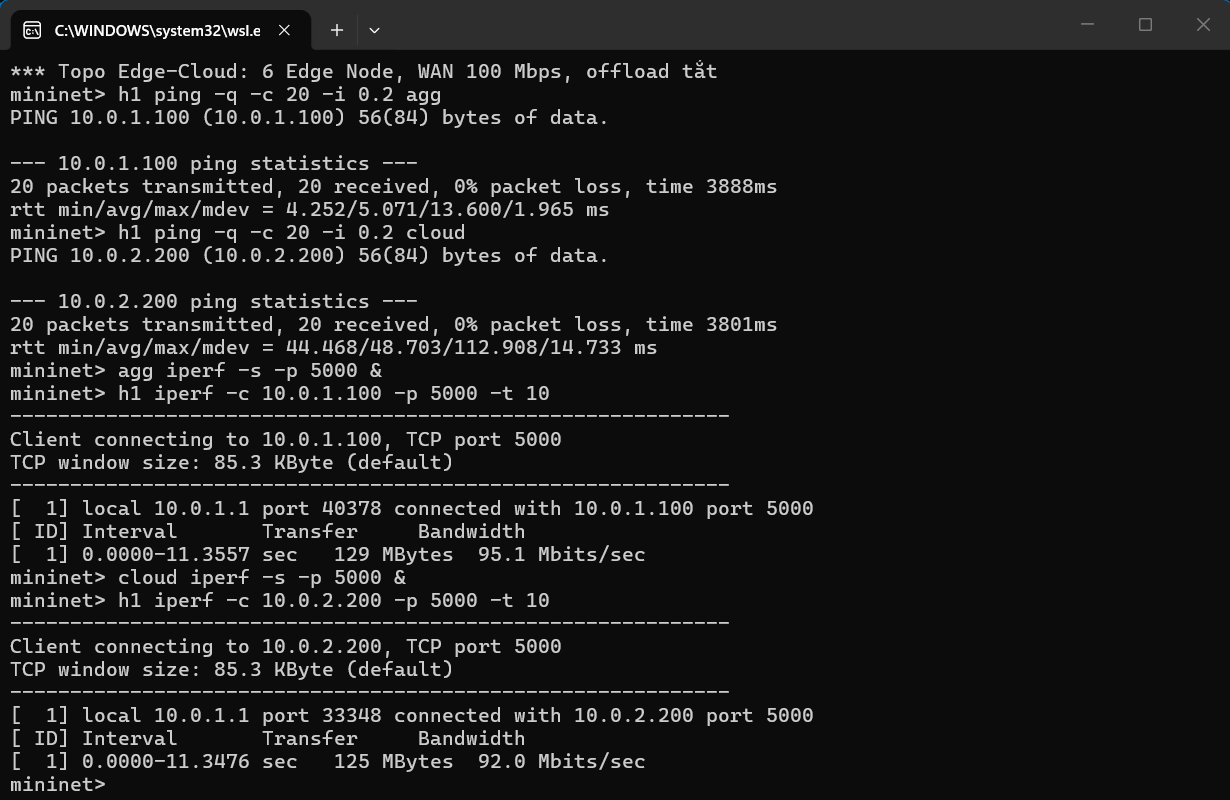
\includegraphics[width=\linewidth]{figs/sanity_wan100.png}
      \hustcaption{ping và iperf trong Mininet CLI, WAN 100 Mbps}
    \end{column}
    \begin{column}{0.46\textwidth}
      \footnotesize
      \begin{tabular}{l c c}
        \toprule
        & \textbf{Kỳ vọng} & \textbf{Đo} \\
        \midrule
        RTT tới \texttt{agg} & 4 ms & 4,25 ms \\
        RTT tới \texttt{cloud} & 44 ms & 44,47 ms \\
        iperf tới \texttt{agg} & 95,6 & 95,1 Mbps \\
        iperf qua WAN 100 & 95,6 & 92,0 Mbps \\
        iperf qua WAN 20 & 19,1 & 18,9 Mbps \\
        \bottomrule
      \end{tabular}
      \vspace{6pt}

      \footnotesize Mọi giá trị không thấp hơn quá 4\% so với $\eta B$: cấu hình băng thông và độ trễ có hiệu lực.
    \end{column}
  \end{columns}
\end{frame}

%% =====================================================================
\section{Kết quả thực nghiệm}
%% =====================================================================

\subsection{Q1 -- Băng thông biên}
\begin{frame}{Q1. Thời gian vòng theo băng thông chặng WAN}{FedAvg thật, $N = 4$, MLP 1,2 MB, Cloud, 20 ms, không mất gói}
  \begin{columns}[c]
    \begin{column}{0.56\textwidth}
      \centering
      \begin{tikzpicture}
        \begin{axis}[
            width=\linewidth, height=5.6cm,
            xmode=log, ymode=log,
            xlabel={Băng thông WAN $B$ (Mbps)}, ylabel={Thời gian (s)},
            xtick={1,2,5,10,20,50,100}, xticklabels={1,2,5,10,20,50,100},
            ytick={0.5,1,2,5,10,20,50,100}, yticklabels={0{,}5,1,2,5,10,20,50,100},
            xmin=0.8, xmax=125, ymin=0.4, ymax=120,
            grid=major, grid style={gray!25},
            tick label style={font=\scriptsize}, label style={font=\scriptsize},
            legend style={font=\scriptsize}, legend pos=north east, legend cell align=left]
          \addplot[thick, HUSTRed, mark=triangle*, mark size=3pt, error bars/.cd, y dir=both, y explicit]
            table[x=bw, y=t_round, y error=t_round_sd, col sep=comma] {data/q1_bw.csv};
          \addlegendentry{$T_{round}$}
          \addplot[thick, hustmain, mark=*, dashed] table[x=bw, y=t_down, col sep=comma] {data/q1_bw.csv};
          \addlegendentry{$T_{down}$}
          \addplot[gray, dashed, domain=0.8:125, samples=2] {1};
          \addlegendentry{$T_{train} = 1$ s}
        \end{axis}
      \end{tikzpicture}
    \end{column}
    \begin{column}{0.42\textwidth}
      \scriptsize
      \begin{tabular}{r c c c}
        \toprule
        $B$ & $T_{round}$ (s) & RTT có tải & TTA \\
        \midrule
        1 & 77,79 & 2054 ms & 1089 s \\
        10 & 8,51 & 200 ms & 119 s \\
        20 & 5,02 & 85 ms & 70 s \\
        100 & 2,32 & 44 ms & 33 s \\
        \bottomrule
      \end{tabular}
      \vspace{4pt}
      \begin{itemize}\footnotesize
        \item $B \le 20$ Mbps: $T_{round} \propto 1/B$, pha tải xuống dùng gần hết băng thông
        \item $B \ge 50$ Mbps: phần cố định (train, slow start) chiếm ưu thế
        \item \textbf{Bufferbloat}: RTT lên 2 s ở 1 Mbps (gấp 46 lần)
        \item $T^* = 10$ s cần $B \gtrsim 9$ Mbps
      \end{itemize}
    \end{column}
  \end{columns}
\end{frame}

\begin{frame}{Q1. Nhiều Edge Node chia chung link vào Aggregator}{Kịch bản K1: Aggregator tại biên, khối 10 MB mỗi chiều, $N = 2..6$}
  \begin{columns}[c]
    \begin{column}{0.54\textwidth}
      \centering
      \begin{tikzpicture}
        \begin{axis}[
            width=\linewidth, height=5.4cm,
            xlabel={Số Edge Node $N$}, ylabel={Thời gian (s)},
            xmin=1.8, xmax=6.2, xtick={2,3,4,5,6}, ymin=0,
            grid=major, grid style={gray!25},
            tick label style={font=\scriptsize}, label style={font=\scriptsize},
            legend style={font=\scriptsize}, legend pos=north west, legend cell align=left]
          \addplot[thick, HUSTRed, mark=triangle*, error bars/.cd, y dir=both, y explicit]
            table[x=n, y=t_round, y error=t_round_sd, col sep=comma] {data/measured_K1_edge_full.csv};
          \addlegendentry{$T_{round}$}
          \addplot[thick, hustmain, mark=*, dashed] table[x=n, y=t_down, col sep=comma] {data/measured_K1_edge_full.csv};
          \addlegendentry{$T_{down}$}
        \end{axis}
      \end{tikzpicture}
    \end{column}
    \begin{column}{0.43\textwidth}
      \scriptsize
      \begin{tabular}{c c c c}
        \toprule
        $N$ & $T_{round}$ đo & gộp & mỗi nút \\
         & (s) & (Mbps) & (Mbps) \\
        \midrule
        2 & 4,45 & 91,2 & 45,6 \\
        4 & 7,33 & 94,8 & 23,7 \\
        6 & 9,94 & 92,1 & 15,4 \\
        \bottomrule
      \end{tabular}
      \vspace{4pt}
      \begin{itemize}\footnotesize
        \item Thông lượng gộp đứng yên $\approx \eta B$; mỗi nút chỉ còn $B/N$
        \item Mỗi node thêm vào: vòng dài thêm $\approx 1{,}37$ s
        \item Link nghẽn là \textbf{giao diện mạng của Aggregator}, link truy nhập dư $(N-1)/N$
        \item $T_{down}$ tăng $\approx 0{,}86$ s/node, sát thời gian truyền 10 MB ở $\eta B$
      \end{itemize}
    \end{column}
  \end{columns}
\end{frame}

\subsection{Q2 -- Mất gói và độ trễ}
\begin{frame}{Q2. Mất gói không làm sai mô hình, chỉ kéo giãn thời gian}{14 lần chạy: 90\% ở đúng vòng 14, chuỗi độ chính xác giống hệt nhau tới chữ số thứ tư}
  \begin{columns}[c]
    \begin{column}{0.56\textwidth}
      \centering
      \begin{tikzpicture}
        \begin{axis}[
            width=\linewidth, height=5.6cm,
            xlabel={Thời gian thực (s)}, ylabel={Độ chính xác},
            xmin=0, xmax=640, ymin=0.60, ymax=0.92, xtick distance=100,
            yticklabel={\pgfmathparse{\tick*100}\pgfmathprintnumber{\pgfmathresult}\%},
            grid=major, grid style={gray!25},
            tick label style={font=\scriptsize}, label style={font=\scriptsize},
            legend style={font=\tiny}, legend pos=south east, legend cell align=left]
          \addplot[thick, hustmain, mark=*, mark size=1.2pt] table[x=time, y=acc, col sep=comma] {data/q2_curve_Q2_loss0.csv};
          \addlegendentry{$p = 0$, RTT 44 ms}
          \addplot[thick, teal, mark=square*, mark size=1.2pt] table[x=time, y=acc, col sep=comma] {data/q2_curve_Q2_loss1.csv};
          \addlegendentry{$p = 1\%$, RTT 44 ms}
          \addplot[thick, HUSTOrange, mark=triangle*, mark size=1.5pt] table[x=time, y=acc, col sep=comma] {data/q2_curve_Q2_loss5.csv};
          \addlegendentry{$p = 5\%$, RTT 44 ms}
          \addplot[thick, HUSTRed, mark=diamond*, mark size=1.5pt] table[x=time, y=acc, col sep=comma] {data/q2_curve_Q2_d100_l1.csv};
          \addlegendentry{$p = 1\%$, RTT 204 ms}
          \addplot[gray, dashed, domain=0:640, samples=2] {0.9};
          \addlegendentry{mục tiêu 90\%}
        \end{axis}
      \end{tikzpicture}
    \end{column}
    \begin{column}{0.42\textwidth}
      \scriptsize
      \begin{tabular}{c c c c}
        \toprule
        $p$ (\%) & $T_{round}$ (s) & truyền lại & TTA (s) \\
        \midrule
        0 & 2,26 & 0,00\% & 32,5 \\
        0,5 & 6,22 & 0,48\% & 83,1 \\
        1 & 8,89 & 1,00\% & 120,2 \\
        2 & 12,49 & 1,99\% & 172,2 \\
        5 & 22,98 & 5,08\% & 317,1 \\
        \bottomrule
      \end{tabular}
      \vspace{4pt}
      \begin{itemize}\footnotesize
        \item Chỉ 0,5\% mất gói: vòng chậm 2,8 lần; 5\%: chậm \textbf{10,2 lần}
        \item $p$ tăng 10 lần $\to T_{down}$ tăng 4,1 lần (Mathis: $\sqrt{10} \approx 3{,}2$)
        \item Tăng nhanh hơn Mathis do timeout RTO khi $p$ lớn
      \end{itemize}
    \end{column}
  \end{columns}
\end{frame}

\begin{frame}{Q2. Độ trễ nhân lên tác hại của mất gói}{WAN 100 Mbps, $N = 4$, $d_{WAN}$ = 5, 20, 50, 100 ms}
  \begin{columns}[c]
    \begin{column}{0.54\textwidth}
      \centering
      \begin{tikzpicture}
        \begin{axis}[
            width=\linewidth, height=5.4cm,
            xlabel={RTT cơ sở (ms)}, ylabel={$T_{round}$ (s)},
            xmin=0, xmax=215, ymin=0, xtick={14,44,104,204},
            grid=major, grid style={gray!25},
            tick label style={font=\scriptsize}, label style={font=\scriptsize},
            legend style={font=\scriptsize}, legend pos=north west, legend cell align=left]
          \addplot[hustmain, mark=*, thick] coordinates {(14,1.823) (44,2.119) (104,2.843) (204,4.342)};
          \addlegendentry{$p = 0$ (chạy lại)}
          \addplot[HUSTRed, mark=triangle*, thick] coordinates {(14,3.733) (44,9.135) (104,17.755) (204,31.539)};
          \addlegendentry{$p = 1\%$}
        \end{axis}
      \end{tikzpicture}
    \end{column}
    \begin{column}{0.43\textwidth}
      \begin{itemize}\footnotesize
        \item $p = 1\%$: RTT 14 $\to$ 204 ms làm $T_{round}$ tăng \textbf{8,4 lần}, TTA từ 51 s lên \textbf{436 s}
        \item 1\% mất gói ở RTT 44 ms $\approx$ hạ băng thông sạch 100 $\to$ 10 Mbps
      \end{itemize}
      \begin{alertblock}{Sai số cấu hình đã phát hiện}
        \footnotesize Giới hạn 200 gói của netem tính cả gói đang bị giữ để tạo trễ, nên đường 50/100 ms bị chặn ở 48/24 Mbps. Lần đo đầu cho 6,2 và 10,7 s; chạy lại với giới hạn đúng: \textbf{2,84 và 4,34 s}.
      \end{alertblock}
    \end{column}
  \end{columns}
\end{frame}

\subsection{Q3 -- Overhead và triển khai biên}
\begin{frame}{Q3. Overhead truyền thông đo từ pcap}{20 vòng FedAvg, $N = 4$: 192,7 MB trọng số hữu ích mỗi lần chạy}
  \begin{columns}[c]
    \begin{column}{0.56\textwidth}
      \scriptsize
      \begin{tabular}{l c c c c}
        \toprule
        \textbf{Kịch bản} & \textbf{Trên dây} & \textbf{Hiệu suất} & \textbf{ACK} & \textbf{Truyền lại} \\
        & (MB) & byte (\%) & (\%) & (\%) \\
        \midrule
        $p = 0$, 20 ms & 206,3 & 93,40 & 2,33 & 0,00 \\
        $p = 0{,}5\%$ & 207,2 & 93,01 & 2,27 & 0,48 \\
        $p = 1\%$ & 208,3 & 92,50 & 2,30 & 1,00 \\
        $p = 2\%$ & 210,5 & 91,56 & 2,31 & 1,99 \\
        $p = 5\%$ & 217,9 & 88,44 & 2,57 & 5,08 \\
        $p = 0$, 100 ms & 210,9 & 91,38 & 2,16 & 2,33 \\
        \bottomrule
      \end{tabular}
      \vspace{6pt}

      \begin{columns}
        \column{0.33\linewidth}\kpi{93,4\%}{byte là trọng số}
        \column{0.33\linewidth}\kpi{4,3\%}{header L2--L4 dữ liệu}
        \column{0.33\linewidth}\kpi{0,003\%}{header FLSync}
      \end{columns}
    \end{column}
    \begin{column}{0.41\textwidth}
      \begin{itemize}\footnotesize
        \item Byte truyền lại $\approx$ tỉ lệ mất gói: TCP + SACK chỉ gửi lại đúng đoạn mất
        \item Header FLSync kể cả khung riêng 86 byte: chỉ 0,014\% byte trên dây
      \end{itemize}
      \begin{alertblock}{Phát hiện chính}
        Ở $p = 5\%$: số byte chỉ tăng \textbf{5,6\%} nhưng thời gian vòng tăng \textbf{10 lần}.\\
        Chi phí của mạng biên nằm ở \emph{thời gian chờ} do điều khiển tắc nghẽn, không nằm ở số byte.
      \end{alertblock}
    \end{column}
  \end{columns}
\end{frame}

\begin{frame}{Q3. Nén bản cập nhật và vị trí Aggregator}{Khối 10 MB xuống; chiều lên 10 MB hoặc 1 MB (nén 1/10)}
  \begin{columns}[c]
    \begin{column}{0.54\textwidth}
      \centering
      \begin{tikzpicture}
        \begin{axis}[
            width=\linewidth, height=5.4cm,
            xlabel={Số Edge Node $N$}, ylabel={$T_{round}$ (s)},
            xmin=1.8, xmax=6.2, xtick={2,3,4,5,6}, ymin=0,
            grid=major, grid style={gray!25},
            tick label style={font=\scriptsize}, label style={font=\scriptsize},
            legend style={font=\tiny}, legend pos=north west, legend cell align=left]
          \addplot[thick, hustmain, mark=*] table[x=n, y=t_round, col sep=comma] {data/measured_K1_edge_full.csv};
          \addlegendentry{Edge, 100 Mbps}
          \addplot[thick, HUSTOrange, mark=square*] table[x=n, y=t_round, col sep=comma] {data/measured_K3_cloud_full.csv};
          \addlegendentry{Cloud, 100 Mbps}
          \addplot[thick, HUSTRed, mark=triangle*] table[x=n, y=t_round, col sep=comma] {data/measured_K3_cloud20_full.csv};
          \addlegendentry{Cloud, 20 Mbps}
        \end{axis}
      \end{tikzpicture}
    \end{column}
    \begin{column}{0.43\textwidth}
      \textbf{Nén 1/10 chiều lên} ($N = 6$, đo)
      \begin{itemize}\footnotesize
        \item Edge: $T_{round}$ 9,94 $\to$ 6,17 s (\textbf{$-$38\%})
        \item Cloud: 11,80 $\to$ 7,52 s (\textbf{$-$36\%})
        \item Qua WAN, nén giảm $d_{trans}$ nhưng không giảm số RTT slow start; pha xuống 10 MB trở thành phần chính
      \end{itemize}
      \textbf{Edge hay Cloud?}
      \begin{itemize}\footnotesize
        \item WAN 100 Mbps: Cloud chậm hơn 0,4--1,9 s/vòng
        \item WAN 20 Mbps: Cloud chậm hơn \textbf{4,9 lần} (48,4 vs 9,9 s)
      \end{itemize}
    \end{column}
  \end{columns}
\end{frame}

\subsection{Phân tích gói tin}
\begin{frame}{Wireshark: slow start lặp lại và chia băng thông}{Bản bắt gói xác nhận các cơ chế TCP dùng để giải thích số đo}
  \begin{columns}[T]
    \begin{column}{0.49\textwidth}
      \centering
      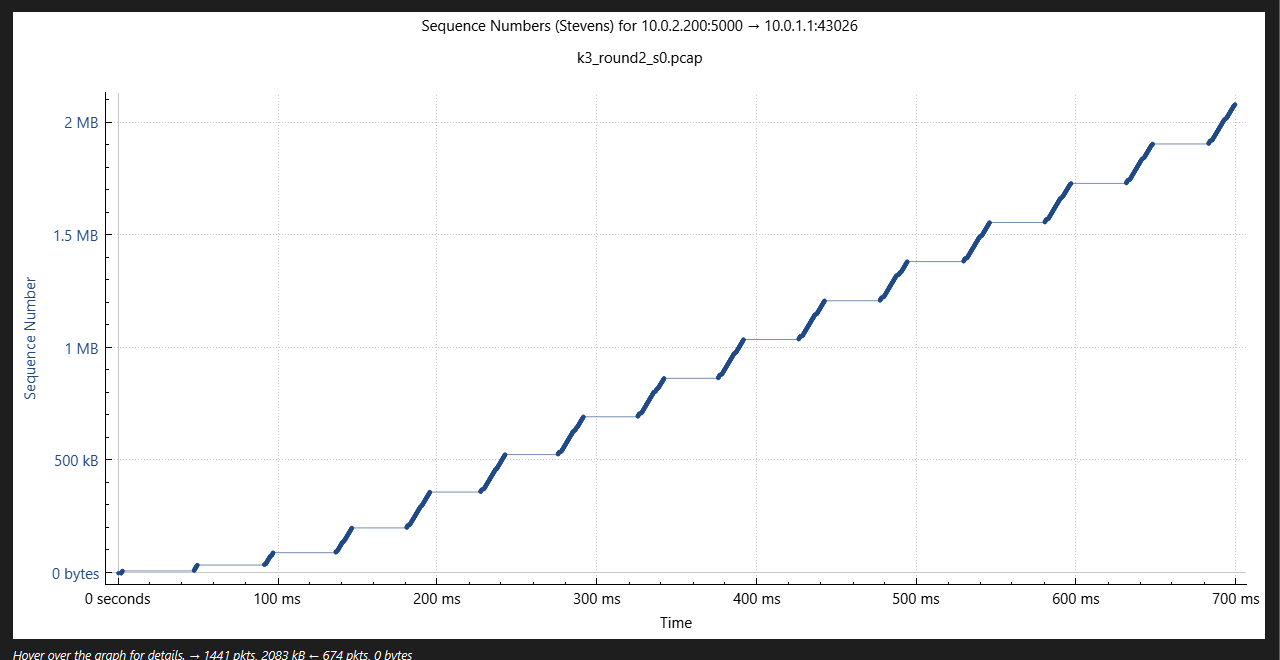
\includegraphics[width=\linewidth,height=3.6cm,keepaspectratio]{figs/ws_stevens.png}
      \hustcaption{Stevens graph, luồng cloud $\to$ h1, đầu vòng 2 (K3)}
      \footnotesize Loạt gói cách nhau 1 RTT: \textbf{10, 18, 38, 76, 110}, rồi 115--121. Dù giữ kết nối TCP, sau 1 s nghỉ $cwnd$ về IW = 10.
    \end{column}
    \begin{column}{0.49\textwidth}
      \centering
      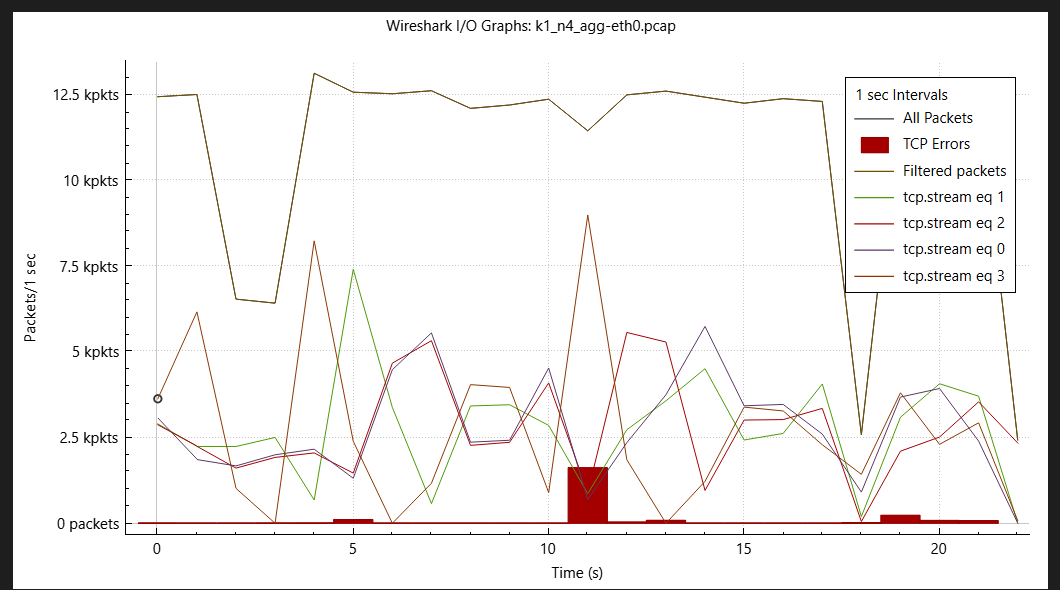
\includegraphics[width=\linewidth,height=3.6cm,keepaspectratio]{figs/ws_io.png}
      \hustcaption{I/O Graph bốn luồng chia link tới Aggregator (K1)}
      \footnotesize Tổng giữ $\approx$ 94--95 Mbps, nhưng từng luồng dao động 0--8,2 MB/s (chia đều chỉ 2,95 MB/s; Jain thấp nhất 0,61): các luồng kết thúc lệch nhau $\Delta$.
    \end{column}
  \end{columns}
\end{frame}

\begin{frame}{Wireshark: header FLSync và gói đi qua Edge Gateway}{}
  \begin{columns}[T]
    \begin{column}{0.49\textwidth}
      \centering
      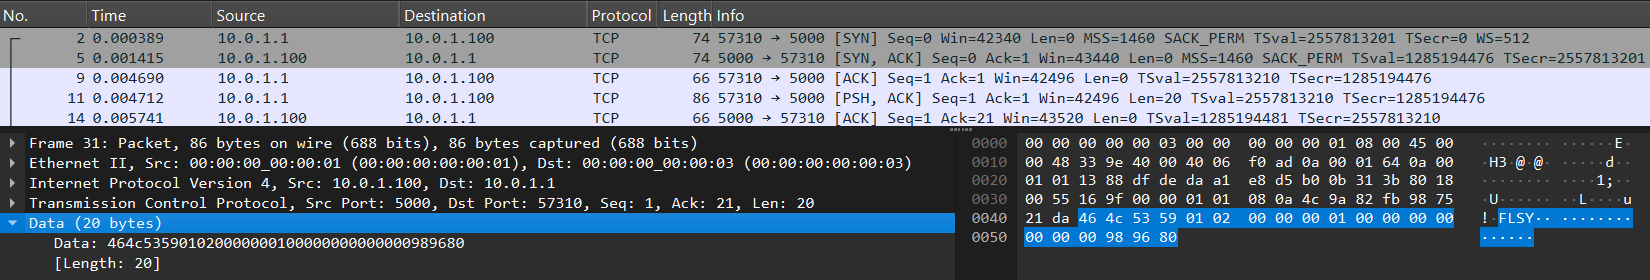
\includegraphics[width=\linewidth,height=3.5cm,keepaspectratio]{figs/ws_hdr.png}
      \hustcaption{Header FLSync của GLOBAL vòng 1}
      \footnotesize \texttt{46 4C 53 59} (FLSY) \texttt{01} \texttt{02} (GLOBAL) \texttt{00000001} (vòng 1) \texttt{0000} (server) \texttt{0000000000989680} (10\,000\,000 B). Đoạn dữ liệu đều dài 1448 B.
    \end{column}
    \begin{column}{0.49\textwidth}
      \centering
      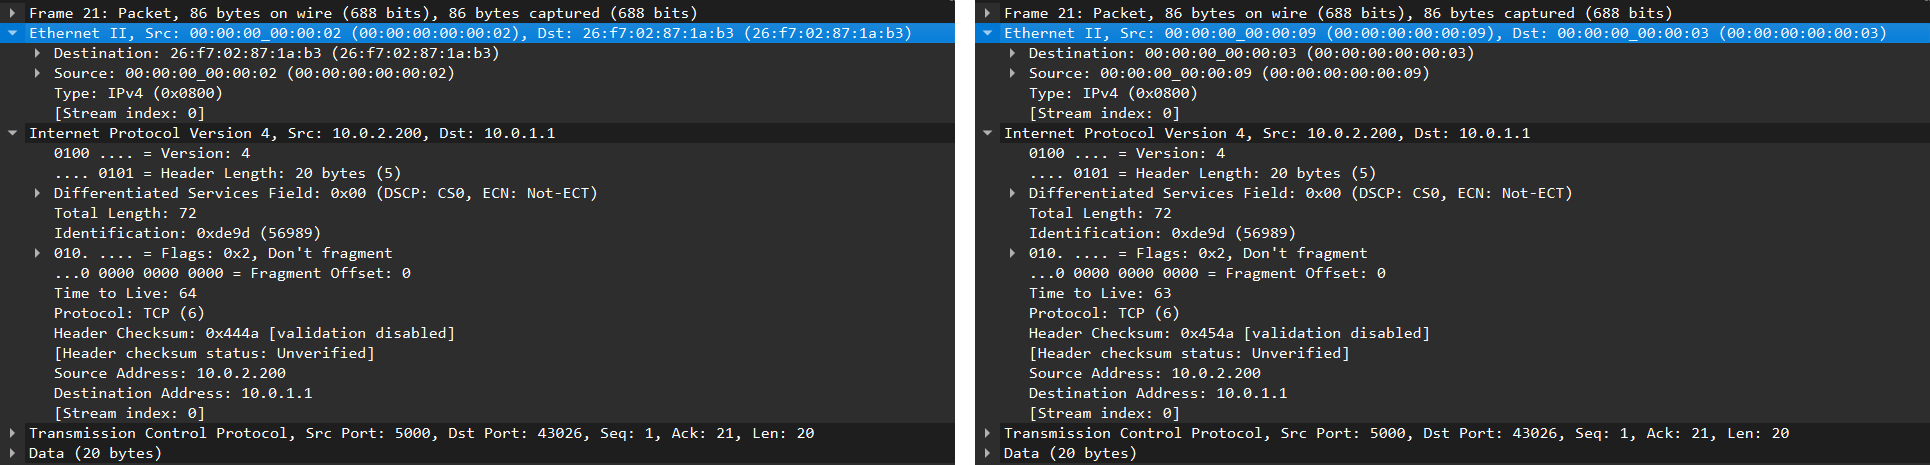
\includegraphics[width=\linewidth,height=3.5cm,keepaspectratio]{figs/ws_router.png}
      \hustcaption{Cùng một gói trước và sau r1}
      \footnotesize Cùng ID \texttt{0xde9d}, cùng IP nguồn/đích; TTL $64 \to 63$, checksum tính lại, cả hai MAC được thay. 343 gói \emph{TCP Retransmission} ($\approx$0,13\%) do hàng đợi 200 gói tràn theo đợt.
    \end{column}
  \end{columns}
\end{frame}

\subsection{Tổng hợp}
\begin{frame}{Tóm tắt kết quả ba câu hỏi nghiên cứu}{}
  \footnotesize
  \begin{tabularx}{\textwidth}{c >{\raggedright\arraybackslash}X >{\raggedright\arraybackslash}X}
    \toprule
    & \textbf{Kết quả đo} & \textbf{Giải thích} \\
    \midrule
    \textbf{Q1} & $T_{round} \propto 1/B$ khi $B \le 20$ Mbps: 77,8 s (1 Mbps), 8,5 s (10 Mbps), 2,3 s (100 Mbps). RTT có tải lên 2 s ở 1 Mbps. Mỗi node thêm: $+1{,}37$ s/vòng (10 MB) & Pha tải xuống dùng gần hết băng thông; link vào Aggregator bão hoà, mỗi nút chỉ nhận $B/N$; hàng đợi 200 gói gây bufferbloat ở đường hẹp \\
    \midrule
    \textbf{Q2} & 90\% ở vòng 14 trong mọi lần chạy. TTA 32,5 $\to$ 317 s khi $p$: 0 $\to$ 5\%; 51 $\to$ 436 s khi RTT 14 $\to$ 204 ms ($p = 1\%$) & TCP truyền lại đủ; thông lượng giảm theo $\sqrt{p}$ và RTT (Mathis), thêm timeout; không mất gói, RTT 44 $\to$ 204 ms chỉ làm vòng dài gấp 2 \\
    \midrule
    \textbf{Q3} & Hiệu suất byte 93,4\% (88,4\% khi $p = 5\%$). Nén 1/10: $-$36--38\% $T_{round}$. Edge nhanh hơn Cloud 4,9 lần khi WAN 20 Mbps & SACK chỉ gửi lại đoạn mất; nén không giảm số RTT slow start; các luồng tải xuống kết thúc lệch nhau \\
    \bottomrule
  \end{tabularx}
\end{frame}

%% =====================================================================
\section{Kết luận}
%% =====================================================================

\begin{frame}{Kết luận và khuyến nghị}{Chi phí thật của mạng biên đối với FL nằm ở thời gian chờ, không nằm ở số byte}
  \begin{columns}[T]
    \begin{column}{0.50\textwidth}
      \textbf{Đã thực hiện}
      \begin{itemize}\small
        \item Topo Edge--Cloud trên Mininet, gateway kiêm firewall, WAN cấu hình được
        \item Giao thức FLSync trên TCP, FedAvg với MLP 1,2 MB
        \item 46 lần chạy tự động: băng thông, mất gói, độ trễ, số nút, nén, vị trí Aggregator
        \item Phân tích pcap bằng Wireshark để giải thích số đo
      \end{itemize}
    \end{column}
    \begin{column}{0.46\textwidth}
      \textbf{Khuyến nghị khi đưa FL ra biên}
      \begin{enumerate}\small
        \item Đặt Aggregator tại biên khi đường lên cloud hẹp, xa hoặc mất gói
        \item Nén bản cập nhật khi băng thông là điểm nghẽn (nén cả chiều xuống)
        \item Cấu hình TCP và hàng đợi: tắt \texttt{slow\_start\_after\_idle}, dùng AQM, thử BBR
        \item Tăng băng thông vào Aggregator khi tăng số nút
      \end{enumerate}
    \end{column}
  \end{columns}
\end{frame}

\begin{frame}{Hướng phát triển}{}
  \begin{itemize}
    \item Thay FLSync bằng gRPC (HTTP/2) hoặc MQTT, đo chi phí thêm của các lớp giao thức
    \item Tắt \texttt{tcp\_slow\_start\_after\_idle}, thử BBR hoặc QUIC để bỏ slow start lặp lại mỗi vòng
    \item Tổng hợp phân cấp: Edge Aggregator gom $N$ bản rồi chỉ gửi một bản lên Cloud
    \item Mất gói theo cụm (Gilbert--Elliott), Edge Node không đồng nhất, bỏ qua bản cập nhật tới muộn
    \item Dữ liệu thật, chia non-IID, mô hình lớn hơn (CNN trên PyTorch)
    \item Chạy lại Q2 có mất gói và K3 với hàng đợi netem đã sửa; AQM (CoDel, fq\_codel) để giảm bufferbloat
  \end{itemize}
\end{frame}

\begin{hustreferencesframe}[from=1, to=8]
\end{hustreferencesframe}


\begin{hustdarkframe}
  \centering
  \vspace*{0.2\paperheight}
  {\Huge\bfseries\color{white} CẢM ƠN CÔ VÀ CÁC BẠN\\ĐÃ LẮNG NGHE!\par}
  \vspace{1.5em}
  {\large\color{white!85} Hỏi \& đáp\par}
\end{hustdarkframe}

\end{document}
